\chapter{Verificación y validación}
\label{CapituloPruebas}
\par En este capítulo se exponen los diferentes ciclos de verificación y validación llevados adelante durante el desarrollo de este proyecto. Según \cite{Press10} ``... La verificación se refiere al conjunto de tareas que garantizan que el software implementa correctamente una función específica. La validación es un conjunto diferente de tareas que aseguran que el software que se construye sigue los requerimientos del cliente.''.

\par En primer lugar son presentadas las inspecciones realizadas sobre el sistema durante su desarrollo. A continuación, se presentan los resultados de una prueba de validación donde los requerimientos establecidos se validan confrontándose con el sistema que se construyó. Luego, son expuestas una serie pruebas del sistema, aplicadas sobre el producto final con el objetivo de asegurar la correcta ejecución y despliegue de resultados. Finalmente, son exhibidas pruebas de campo realizadas a partir de diferentes experimentos de maceración, monitoreados por el sistema, de manera de validar que el mismo se comporte según lo esperado.

\section{Verificación: Inspecciones del sistema}

\par Durante el ciclo de vida del proyecto, de forma constante y repetitiva, fueron analizados los requerimientos funcionales y no funcionales, así como las especificaciones formuladas durante el diseño. De esta forma, luego de implementar e integrar funcionalidades en los componentes desarrollados, se analizó la documentación de forma de asegurar que se cumpliera con todos los requisitos y requerimientos.

\par Junto al avance del desarrollo de los componentes fueron aplicadas las siguientes pruebas estáticas de forma de comprobar que las funcionalidades cumplieran su objetivo de manera individual e integral:

\begin{itemize}
    \item Pruebas en componente de hardware: recolección de datos de sensores; inserción en base de datos.
    \item Pruebas de interfaz Hardware-Software: verificación de funcionamiento de la \textit{REST API} desarrollada. La \textit{REST API} fue probada utilizando la herramienta \textit{Postman}\footnote{\textit{Postman}, Entorno de desarrollo de \textit{APIs} \url{https://www.getpostman.com/}}. Mediante esta herramienta se proveyeron datos a la \textit{REST API} de la misma forma en que luego serían provistas por la aplicación, así fueron identificados y corregidos distintos fallos.
    \item Pruebas de la aplicación: verificación de funcionalidades, de manera individual, imprimiendo en el retorno del sistema (\textit{Log}) del entorno de desarrollo \textit{AndroidStudio} diferentes variables de control, verificando así el correcto funcionamiento. En forma adicional, fueron probadas todas las funcionalidades que interactúan de forma integral con el sistema (métodos de interacción con la \textit{REST API}).
\end{itemize}

\par A continuación se presentan las pruebas de ``cálculo de insumos'' y ``cálculo de rendimiento'', llevadas a cabo de manera de verificar su correcto funcionamiento.

\subsection{Cálculo de insumos}
\par Se procedió a realizar la verificación de los cálculos de insumos implementados mediante el uso de recetas provistas por los directores. Estas recetas incluyen cantidades obtenidas mediante la aplicación de cálculos en los que se asume el extracto potencial de la malta como del 100\%. Por tanto, las cantidades diferirán con las aquí calculadas entre un 15\% y un 30\% dado que para el cálculo son utilizados los extractos potenciales reales de las maltas, los cuales varían entre un 70-85\%. Tomando en cuenta lo antes mencionado, se consideran como válidos los cálculos que se encuentren dentro de estos intervalos.

\par En la Tabla \ref{tab:TablaRecetaExperimentos}, se presentan las recetas y la comparativa de los valores de insumos allí presentes con los obtenidos por la aplicación.

\begin{longtable}{|p{1.8cm}|p{1.8cm}|p{1.8cm}|p{1.9cm}|p{1.7cm}|p{2cm}|p{2cm}|}
    \hline
    Nombre Receta & Granos & Porcentaje & Volumen & Densidad Objetivo & Insumo Receta & Insumo Calculado \\
    \hline
    \hline
    \endfirsthead
    
    \hline
    \endfoot
    
    \hline
    \multicolumn{7}{|c|}{Continuación de la Tabla \ref{tab:TablaRecetaExperimentos}}\\
    \hline
    Nombre Receta & Granos & Porcentaje & Volumen & Densidad Objetivo & Insumo Receta & Insumo Calculado \\
    \hline
    \hline
    \endhead
    
    \hline
    \caption{Recetas empleadas para experimentos \label{tab:TablaRecetaExperimentos}}\\
    \endlastfoot
    
    %content
    \multirow{2}{2cm}{English Pale Ale} & Pilsen &\multicolumn{1}{c|}{86\%}  &\multirow{2}{2cm}{48.6 litros}  &\multirow{2}{2cm}{1.090} & \multicolumn{1}{c|}{14.04 Kg.} & \multicolumn{1}{c|}{17.34 Kg.}\\
         & Munich & \multicolumn{1}{c|}{14\%} & & &\multicolumn{1}{c|}{2.35 Kg.} &\multicolumn{1}{c|}{2.86 Kg.} \\
        \hline
        \multirow{3}{2cm}{American Blonde Ale} & Pilsen &\multicolumn{1}{c|}{86\%}  &\multirow{3}{2cm}{38.7 litros}  &\multirow{3}{2cm}{1.080} & \multicolumn{1}{c|}{9.47 Kg.} & \multicolumn{1}{c|}{12.28 Kg.}\\
         & Malted Wheat & \multicolumn{1}{c|}{7\%} & & &\multicolumn{1}{c|}{0.87 Kg.} &\multicolumn{1}{c|}{0.96 Kg.}\\ 
         & Carapils & \multicolumn{1}{c|}{7\%} & & & \multicolumn{1}{c|}{0.87 Kg.} &\multicolumn{1}{c|}{1.12 Kg.} \\
        \hline
        \multirow{5}{2cm}{New England IPA} & Pilsen &\multicolumn{1}{c|}{80\%}  &\multirow{5}{2cm}{43.7 litros}  &\multirow{5}{2cm}{1.090} & \multicolumn{1}{c|}{9.6 Kg.} & \multicolumn{1}{c|}{14.51 Kg.}\\
         & Oats & \multicolumn{1}{c|}{10\%} & & &\multicolumn{1}{c|}{1.26 Kg.} &\multicolumn{1}{c|}{1.84 Kg.} \\
        & Carapils & \multicolumn{1}{c|}{4\%} & & &\multicolumn{1}{c|}{0.61 Kg.} &\multicolumn{1}{c|}{0.98 Kg.} \\
        & Wheat & \multicolumn{1}{c|}{3\%} & & &\multicolumn{1}{c|}{0.5 Kg.} &\multicolumn{1}{c|}{0.7 Kg.} \\
        & Corn Sugar & \multicolumn{1}{c|}{3\%} & & &\multicolumn{1}{c|}{0.6 Kg.} &\multicolumn{1}{c|}{0.6 Kg.} \\
        \hline
        \multirow{4}{2cm}{Session IPA} & Pilsen &\multicolumn{1}{c|}{62\%}  &\multirow{4}{2cm}{40.5 litros}  &\multirow{4}{2cm}{1.070} & \multicolumn{1}{c|}{7.69 Kg.} & \multicolumn{1}{c|}{8.11 Kg.}\\
         & Cara Munich & \multicolumn{1}{c|}{23.5\%} & & &\multicolumn{1}{c|}{2.9 Kg.} &\multicolumn{1}{c|}{3.47 Kg.} \\
        & Crystal Munich & \multicolumn{1}{c|}{5.5\%} & & &\multicolumn{1}{c|}{0.73 Kg.} &\multicolumn{1}{c|}{0.83 Kg.} \\
        & Carapils & \multicolumn{1}{c|}{9\%} & & &\multicolumn{1}{c|}{1.11 Kg.} &\multicolumn{1}{c|}{1.32 Kg.} \\
        \hline
        \multirow{8}{2cm}{Hopfen - Weizen} & Pilsen &\multicolumn{1}{c|}{44.44\%}  &\multirow{8}{2cm}{44.15 litros}  &\multirow{8}{2cm}{1.070} & \multicolumn{1}{c|}{5.99 Kg.} & \multicolumn{1}{c|}{6.33 Kg.}\\
         & Malted Wheat & \multicolumn{1}{c|}{33.33\%} & & &\multicolumn{1}{c|}{4.5 Kg.} &\multicolumn{1}{c|}{4.58 Kg.} \\
         & Carapils & \multicolumn{1}{c|}{7.4\%} & & &\multicolumn{1}{c|}{0.99 Kg.} &\multicolumn{1}{c|}{1.19 Kg.} \\
         & Caramel Wheat & \multicolumn{1}{c|}{3.7\%} & & &\multicolumn{1}{c|}{0.49 Kg.} &\multicolumn{1}{c|}{0.61 Kg.} \\
         & Biscuit & \multicolumn{1}{c|}{3.7\%} & & &\multicolumn{1}{c|}{0.49 Kg.} &\multicolumn{1}{c|}{0.54 Kg.} \\
         & Ruby & \multicolumn{1}{c|}{3\%} & & &\multicolumn{1}{c|}{0.4 Kg.} &\multicolumn{1}{c|}{0.44 Kg.} \\
         & Munich Best Malz & \multicolumn{1}{c|}{2.2\%} & & &\multicolumn{1}{c|}{0.297 Kg.} &\multicolumn{1}{c|}{0.32 Kg.} \\
         & Chocolate & \multicolumn{1}{c|}{1.5\%} & & &\multicolumn{1}{c|}{0.2 Kg.} &\multicolumn{1}{c|}{0.24 Kg.} \\
        \hline
    
\end{longtable}

\par Siendo que los valores provenientes de los cálculos y recetas, presentados en la Tabla \ref{tab:TablaRecetaExperimentos}, difieren dentro del rango antes mencionado debido a la inclusión del extracto potencial de malta en el cálculo, se asume como exitosa esta prueba. %satisfacen los objetivos antes presentados, 

\subsection{Cálculo de rendimiento}
\par Para verificar la fórmula de rendimiento, se ingresaron al cálculo de rendimiento valores de densidad objetivo, volumen y cantidad de insumos utilizados y proporcionados por el cálculo de insumos. Se verifica el correcto funcionamiento si la ecuación expresa el mismo rendimiento que el utilizado para el cálculo de insumos.

\begin{table}[H]
    \centering
    \begin{tabularx}{\textwidth}{|X|X|X|X|X|X|}
        \hline
        Densidad & Volumen & Total de Insumos [kg] & Total de extracto [kg] & Rendimiento utilizado & Rendimiento Calculado \\
        \hline
        \hline
        1.070 & 1.1 litros & 0.366 & 0.288 & 0.70 & 0.7038\\ \hline
        1.070 & 40.55 litros & 13.73 & 10.98 & 0.70 & 0.7054 \\ \hline
        1.090 & 43.7 litros & 18.62 & 14.98 & 0.70 & 0.6976 \\ \hline
    \end{tabularx}
    \caption{Tabla de validación del cálculo de rendimiento}
    \label{tab:rendimiento}
\end{table}

\par Como puede observarse en la Tabla \ref{tab:rendimiento} el error de aproximación es menor al 0,7\% lo cual considera a los valores obtenidos como aceptables. La desviación se debe a los redondeos utilizados en cada cálculo. 

\section{Pruebas de validación}
 \par En este apartado, se valida que el sistema cumple con los requerimientos especificados en las Tablas \ref{reqFunc} y \ref{reqNoFunc}. A continuación, se presenta la Tabla \ref{tab:TablaChequeoRequerimientos} donde junto a al identificador de cada requerimiento, se presenta un breve texto mediante el cual se valida que el sistema lo satisface.

 \begin{longtable}{|p{3cm}|p{11cm}|}
    \hline
    \multicolumn{2}{| c |}{\textbf{Tabla de verificación de requerimientos}}\\
    \hline
    \multicolumn{1}{| c |}{Requerimiento} &\multicolumn{1}{| c |}{Verificación}\\
    \hline
    \hline
 \endfirsthead
 
 \hline
    \multicolumn{2}{|c|}{Continuación de la tabla de verificación de requerimientos}\\
    \hline
    \multicolumn{1}{| c |}{Requerimiento} &\multicolumn{1}{| c |}{Verificación}\\
    \hline
 \endhead

 \endfoot
 
 \caption{Tabla de validación de requerimientos \label{tab:TablaChequeoRequerimientos}}\\
 \endlastfoot
     
        \multicolumn{1}{|c|}{RF001} & El sistema implementa el uso de sensores de temperatura, pH y temperatura ambiente. Mencionados en el capítulo \ref{CapituloHardware} (\textit{\textbf{Hardware}}). \\
        \hline
        
        \multicolumn{1}{|c|}{RF002} & El sistema implementa el uso de cuatro sensores de temperatura ubicados en distintas posiciones del macerador. El uso de los mismos se menciona en el capítulo \ref{CapituloHardware} (\textit{\textbf{Hardware}}) y posteriormente en este mismo capítulo. \\
        \hline
        
        \multicolumn{1}{|c|}{RF003} & El sistema permite visualizar los datos recolectados por los sensores se este llevando a cabo o no un experimento de maceración. Mencionado en el capítulo \ref{CapituloSoftware} (\textit{\textbf{Software}}). \\
        \hline
        
        \multicolumn{1}{|c|}{RF004} & El sistema a través de la aplicación, permite ingresar todos los datos que caracterizan a una receta de maceración mediante una pantalla destinada a este fin. Mencionado en el capítulo \ref{CapituloSoftware} (\textit{\textbf{Software}}).  \\
        \hline
        
        \multicolumn{1}{|c|}{RF005} & El sistema emite alertas gráficas y sonoras ante desvíos entre los valores planificados y los obtenidos durante un experimento de macerado. Mencionado en el capítulo \ref{CapituloSoftware} (\textit{\textbf{Software}}). \\
        \hline
        
        \multicolumn{1}{|c|}{RF006}  & El sistema, en particular la aplicación móvil, cuenta con la capacidad de almacenar recetas de maceración, y permite remover una maceración existente junto a todos los experimentos relacionados a ella. Mencionado en el capítulo \ref{CapituloSoftware} (\textit{\textbf{Software}}). \\
        \hline
        
        \multicolumn{1}{|c|}{RF007} & El sistema permite almacenar y eliminar los datos de los experimentos realizados, estos pueden ser gestionados mediante la interfaz gráfica de la aplicación. Mencionado en el capítulo \ref{CapituloSoftware} (\textit{\textbf{Software}}). \\
        \hline
        
        \multicolumn{1}{|c|}{RF008} & El sistema, mediante la aplicación móvil, informa las cantidades de insumos a utilizar para cada receta de maceración. Estos insumos son calculados mediante dos aproximaciones: una estimación teórica y un ajuste empírico de los valores teóricos basados en resultados antes obtenidos. De forma adicional, brinda los cálculos de volumen y temperatura del agua para cada Etapa. Mencionado en el capítulo \ref{CapituloSoftware} (\textit{\textbf{Software}}). \\
        \hline 
        
        \multicolumn{1}{|c|}{RF009} & El sistema provee gráficas de los datos recolectados en cada experimento de maceración ubicados en una única pantalla. De forma adicional, provee gráficas relativas a resultados obtenidos del conjunto de experimentos para una misma receta de maceración. Mencionado en el capítulo \ref{CapituloSoftware} (\textit{\textbf{Software}}). \\
        \hline
        
        \multicolumn{1}{|c|}{RF010} & Luego de tres experimentos de macerado concretados para una misma receta de maceración, el sistema comienza a optimizar los insumos. El resultado de estas optimizaciones es presentado junto a los valores no optimizados en una pantalla destinada a este fin. Mencionado en el capítulo \ref{CapituloSoftware} (\textit{\textbf{Software}}). \\
        \hline
        
        \multicolumn{1}{|c|}{RF011} & Durante un experimento de maceración en curso, el sistema presenta un único valor de temperatura representativo del tanque. Este valor es obtenido aplicando el cálculo de medidas de tendencia central. El sistema permite seleccionar entre tres métodos de cálculo para este valor: media, mediana  y  promedio  de  valores extremos. Mencionado en el capítulo \ref{CapituloSoftware} (\textit{\textbf{Software}}). \\
        \hline
        
        \multicolumn{1}{|c|}{RNF001} & La plataforma elegida para la aplicación, \textit{Android},  se basó en este requerimiento siendo esta la más usada en el mercado Argentino. Mencionado en el capítulo \ref{CapituloHardware} (\textit{\textbf{Hardware}}). \\
        \hline
        
        \multicolumn{1}{|c|}{RNF002} & El sistema produce resultados aceptables para recolectar un conjunto de valores, luego el lapso consumido para el envío de los datos a la aplicación es despreciable por su duración corroborando asi este requerimiento. Mencionado en la sección \textit{\textbf{Pruebas de rendimiento}} del presente capítulo. \\
        \hline
        
        \multicolumn{1}{|c|}{RNF003} & Los datos inherentes a los experimentos realizados se almacenan en los componentes de hardware y software. Mencionado en los capítulos \ref{CapituloHardware} (\textit{\textbf{Hardware}}) y \ref{CapituloSoftware} (\textit{\textbf{Software}}). \\
        \hline
        
        \multicolumn{1}{|c|}{RNF004} & Durante la comunicación entre el componente de software y el componente de hardware, el primero envía una lista con los ID's relativos a los paquetes de datos de mediciones recibidas. Luego, el hardware envía como respuesta todos los paquetes de datos que tenga almacenados cuyos ID's no se encuentren en la lista recibida. De esta manera, se establece un protocolo de comunicación que contempla la ocasional pérdida de paquetes que pudiese sucederse. Mencionado en el capítulo \ref{CapituloHardware} (\textit{\textbf{Hardware}}). \\
        \hline
        
        \multicolumn{1}{|c|}{RNF005} & La comunicación entre el dispositivo móvil y la estación de recolección de datos se realiza mediante tecnología inalámbrica WIFI\textsuperscript{\textregistered}. Mencionado en el capítulo \ref{capituloInterfaz} (\textit{\textbf{Interfaz hardware - software}}).\\
        \hline
        
        \multicolumn{1}{|c|}{RNF006} & Al momento de elegir los diferentes sensores utilizados, se tuvo en cuenta este requerimiento. Mencionado en el capítulo \ref{CapituloHardware} (\textit{\textbf{Hardware}}).\\
        \hline
        
        \multicolumn{1}{|c|}{RNF007} & Al momento de seleccionar la placa electrónica se optó por la placa Raspberry\textsuperscript{\textregistered} ya que de entre sus especificaciones se satisface el mayor número de necesidades que se presentaron de forma comparativa a otras opciones evaluadas. Mencionado en el capítulo \ref{CapituloHardware} (\textit{\textbf{Hardware}}).\\
        \hline
    \end{longtable}

\section{Pruebas del sistema: ejecución y despliegue de resultados}

\par En esta sección se describen las validaciones realizadas a las funcionalidades del sistema mediante distintos tipos de pruebas dinámicas. Según \cite{Press10} ´´La prueba del sistema verifica que todos los elementos se mezclan de manera adecuada y que se logra el funcionamiento/rendimiento global del sistema.''.

\subsection{Pruebas funcionales}

\par La validación del correcto funcionamiento de la aplicación es llevado a cabo mediante la aplicación de pruebas del sistema de tipo ``Entrega''. Según \cite{Som05} ``\ldots Las pruebas de entrega, “pruebas funcionales” o “pruebas de caja negra”, son aquellas en las que sólo interesan las funcionalidades del sistema y no su implementación. En otras palabras, se valida que el sistema satisfaga sus requerimientos \ldots''.
\par Las pruebas son llevadas a cabo a partir del uso de casos de prueba. La definición de los casos de prueba fue realizada a partir de los casos de uso ubicados en el capítulo de ´´Ingeniería de requerimientos''.
\par Las pruebas son ejecutadas por el único usuario del sistema, el fabricante de cerveza artesanal. Al final de cada ficha bajo el título de ``Evidencias'', se ubica un hipervínculo a un vídeo, donde podrá observarse la ejecución de la prueba.

\subsubsection{Fichas de casos de prueba}

\par A continuación son presentadas las fichas de casos de prueba, las cuales incluyen el actor, una breve descripción del propósito de la prueba, las acciones realizadas que incluyó la prueba, el resultado que indica la correcta aprobación y la evidencia que comprueba que las acciones fueron llevadas a cabo.

%----------------- FICHA CASO DE PRUEBA 1 ------------------------

\begin{longtable}{|p{0.6cm}|p{4cm}|p{4.7cm}|p{4.7cm}|}
    \hline
    \multicolumn{4}{| c |}{\textbf{Caso de prueba: Monitorear variables - CP001}}\\
    \hline
    \multicolumn{4}{| l |}{\textbf{Actor de caso de prueba:} Productor de cerveza}\\
    \hline
    \multicolumn{4}{| l |}{\textbf{Propósito}}\\
    \hline
    \multicolumn{4}{|p{0.95\linewidth}|}{Verificar la correcta funcionalidad del dialogo que proporciona los datos siendo recolectados por los sensores de la estación de recolección de datos. Verificar que se despliegan en pantalla los datos antes mencionados.}\\
    \hline
    \endfirsthead
 
    \hline
    \multicolumn{4}{|c|}{Continuación de la Tabla \ref{CasoDePrueba1}}\\
    \hline
    \multicolumn{4}{| l |}{\textbf{Descripción de acciones para las pruebas}}\\
    \hline
    \textbf{\#} & Acciones & Salida esperada & Salida obtenida\\
    \hline
    \endhead
 
    \hline
    \endfoot
 
    \hline
    \multicolumn{4}{| c |}{\textbf{Resultados obtenidos}}\\
    \hline
    \multicolumn{4}{| l |}{\textbf{Resultado}: Aprobado}\\
    \hline
    \multicolumn{4}{| l |}{\textbf{Evidencia}: \url{https://shorturl.me/BauGZ} }\\
    \hline
    \caption{Ficha de caso de prueba CP001\label{CasoDePrueba1}}\\
    \endlastfoot

    \multicolumn{4}{| l |}{\textbf{Descripción de acciones para las pruebas}}\\
    \hline
    \textbf{\#} & Acciones & Salida esperada & Salida obtenida\\
    \hline
    01 & Abrir el panel mediante el botón destinado a ello presente en la pantalla principal & Se abre el panel y se despliegan los datos esperados. & El panel se abrió correctamente y se mostraron luego los datos esperados. \\
    \hline

 \end{longtable}

%----------------- FIN FICHA CASO DE PRUEBA 1------------------------

%----------------- FICHA CASO DE PRUEBA 2------------------------

\begin{longtable}{|p{0.6cm}|p{4cm}|p{4.7cm}|p{4.7cm}|}
    \hline
    \multicolumn{4}{| c |}{\textbf{Caso de prueba: Cargar una maceración - CP002}}\\
    \hline
    \multicolumn{4}{| l |}{\textbf{Actor de caso de prueba:} Productor de cerveza}\\
    \hline
    \multicolumn{4}{| l |}{\textbf{Propósito}}\\
    \hline
    \multicolumn{4}{|p{0.95\linewidth}|}{ Verificar la correcta apertura y funcionalidad de la pantalla destinada para la carga y creación de una nueva maceración.}\\
    \hline
    \endfirsthead
 
    \hline
    \multicolumn{4}{|c|}{Continuación de la Tabla \ref{CasoDePrueba2}}\\
    \hline
    \endhead
 
    \hline
    \endfoot
 
    \hline
    \multicolumn{4}{| c |}{\textbf{Resultados obtenidos}}\\
    \hline
    \multicolumn{4}{| l |}{\textbf{Resultado}: Aprobado}\\
    \hline
    \multicolumn{4}{| l |}{\textbf{Evidencia}: \url{https://shorturl.me/eR1LM} }\\
    \hline
    \caption{Ficha de caso de prueba CP002\label{CasoDePrueba2}}\\
    \endlastfoot

    \multicolumn{4}{| l |}{\textbf{Descripción de acciones para las pruebas}}\\
    \hline
    \textbf{\#} & Acciones & Salida esperada & Salida obtenida\\
    \hline
    01 & Apertura de la pantalla mediante el botón destinado a ello presente en la pantalla principal & Se abre la pantalla con el formulario. & La pantalla se abrió correctamente desplegando en ella el formulario a rellenar. \\
    \hline
    02 & Agregar grano (formulario incompleto), apertura del diálogo y relleno incompleto del formulario & Se abre el diálogo con el formulario. No se agrega el grano y despliega un mensaje de error. & Se abrió el diálogo con el formulario. No se agregó el grano y desplegó un mensaje de error: ``No se pudo insertar el grano porque faltaron completar campos''. \\
    \hline
    03 & Agregar grano (formulario completo), apertura del diálogo y relleno completo del formulario, luego se agrega el mismo pudiendo ver los datos del mismo en el formulario principal & Se abre el diálogo con el formulario, se rellena el mismo y luego es agregado el grano a la lista de granos. & Se abrió el diálogo con el formulario. El grano fue agregado a la lista. \\
    \hline
    04 & Eliminar grano, se abre el menú con la opción de eliminación luego de realizar una presión larga de un grano de la lista. Luego de seleccionada la eliminación en el menú, el mismo es retirado de la lista. & Se abre el menú, se selecciona eliminar y el mismo es removido de la lista. & Se abrió el menú, se seleccionó eliminar y el mismo fue removido de la lista de granos. \\
    \hline
    05 & Agregar nuevo intervalo de medición (formulario incompleto), luego de presionado el botón para este fin se abre un diálogo y se rellena de forma incompleta el formulario.  & No se agrega el intervalo a la lista de intervalos y se despliega un mensaje de error. & Se abrió el diálogo con el formulario. El intervalo no fue agregado a la lista y se desplegó un mensaje de error:``No se pudo insertar el intervalo porque faltaron completar campos''\\
    \hline
    06 & Agregar nuevo intervalo de medición (formulario completo), luego de presionado el botón para este fin se abre un diálogo y se rellena de forma completa el formulario presente en el mismo. & Se abre el diálogo con el formulario y luego es agregado el intervalo a la lista de intervalos. & Se abrió el diálogo con el formulario. El intervalo fue agregado a la lista.\\
    \hline
    07 & Finalizar carga de maceración (formulario principal, grano y/o intervalos no agregados). & Se presiona el botón de confirmación se despliega un error. & Se desplegó un mensaje de error por cada tipo de campo incompleto.\\
    \hline
    08 & Finalizar carga de maceración (formulario principal completo, grano e intervalos agregados, formulario de finalización incompleto), luego de presionado el botón para este fin se despliega un dialogo con un formulario final, se rellena el formulario de forma incompleta. & Se presiona el botón de confirmación y se despliega un error. & Se desplegó un mensaje de error: ``No se guardó, hay algún campo incompleto''.\\
    \hline
    09 & Finalizar carga de maceración (formulario principal completo, grano e intervalos agregados, formulario de finalización completo), luego de presionado el botón para este fin se despliega un dialogo con un formulario final, se rellena el formulario de forma completa. & Se presiona el botón de confirmación, vuelve a la pantalla principal desplegando un mensaje de confirmación. & Volvió a la pantalla principal y desplegó un mensaje de confirmación: ``Maceración correctamente planificada''.\\
    \hline

 \end{longtable}

%----------------- FIN FICHA CASO DE PRUEBA 2------------------------

%----------------- FICHA CASO DE PRUEBA 3------------------------

\begin{longtable}{|p{0.6cm}|p{4cm}|p{4.7cm}|p{4.7cm}|}
    \hline
    \multicolumn{4}{| c |}{\textbf{Caso de prueba: Gestionar maceración - CP003}}\\
    \hline
    \multicolumn{4}{| l |}{\textbf{Actor de caso de prueba:} Productor de cerveza}\\
    \hline
    \multicolumn{4}{| l |}{\textbf{Propósito}}\\
    \hline
    \multicolumn{4}{|p{0.95\linewidth}|}{ Verificar la correcta apertura y funcionalidad de la pantalla destinada a informar y acceder a los experimentos realizados para la maceración seleccionada, consultar información de los insumos que se utilizan, iniciar un nuevo experimento y visualizar datos estadísticos generales y particulares de cada experimento. }\\
    \hline
    \endfirsthead
 
    \hline
    \multicolumn{4}{|c|}{Continuación de la Tabla \ref{CasoDePrueba3}}\\
    \hline
    \endhead
 
    \hline
    \endfoot
 
    \hline
    \multicolumn{4}{| c |}{\textbf{Resultados obtenidos}}\\
    \hline
    \multicolumn{4}{| l |}{\textbf{Resultado}: Aprobado}\\
    \hline
    \multicolumn{4}{| l |}{\textbf{Evidencia}: \url{https://shorturl.me/CBPyJ72} }\\
    \hline
    \caption{Ficha de caso de prueba CP003\label{CasoDePrueba3}}\\
    \endlastfoot

    \multicolumn{4}{| l |}{\textbf{Descripción de acciones para las pruebas}}\\
    \hline
    \textbf{\#} & Acciones & Salida esperada & Salida obtenida\\
    \hline
    01 & Apertura de la pantalla mediante el ítem de la lista de maceraciones presente en la pantalla principal & Se abre la pantalla con la lista de experimentos realizados y botones correspondientes a las opciones de gestión. & La pantalla se abrió correctamente desplegando la lista y las opciones. \\
    \hline
    02 & Eliminar Maceración, apertura del diálogo y selección opción ``Cancelar'' & Se abre el diálogo en el que se despliega un mensaje de advertencia, se cierra el diálogo sin aplicar modificaciones & Se abrió el diálogo con el mensaje: ``¿Está seguro que desea eliminar maceración?'' , el cuadro de dialogo se cerró y no se realizaron modificaciones. \\
    \hline
    03 & Eliminar Maceración, apertura del diálogo y selección opción ``Aceptar'' & Se abre el diálogo en el que se despliega un mensaje de advertencia, se inicia la pantalla principal.  & Se abrió el diálogo con el mensaje ``¿Está seguro que desea eliminar maceración?''. la maceración se eliminó y se inició la pantalla principal. \\
    \hline
    04 & Iniciar Nuevo Experimento & El usuario selecciona la opción ``Iniciar nuevo experimento''. Se abre la pantalla destinada a esta tarea.& Se seleccionó la opción correspondiente y se inició la pantalla.\\
    \hline
    05 & Ver detalles de maceración, luego de presionado el botón correspondiente a esta opción & El usuario selecciona la opción ``Ver Planificación''. Se abre la pantalla destinada a esta tarea.& Se seleccionó la opción correspondiente y se inició la pantalla que indica los valores de los insumos calculados.\\
    \hline
    06 & Ver estadísticas de maceración, Se presiona el botón correspondiente a esta opción. & Se despliega la pantalla de estadísticas históricas de  la maceración.& Se desplegó la pantalla de estadísticas históricas de  la maceración.\\
    \hline
 \end{longtable}

%----------------- FIN FICHA CASO DE PRUEBA 3------------------------

%----------------- FICHA CASO DE PRUEBA 4 ------------------------

\begin{longtable}{|p{0.6cm}|p{4cm}|p{4.7cm}|p{4.7cm}|}
    \hline
    \multicolumn{4}{| c |}{\textbf{Caso de prueba: Iniciar experimento de Maceración - CP004}}\\
    \hline
    \multicolumn{4}{| l |}{\textbf{Actor de caso de prueba:} Productor de cerveza}\\
    \hline
    \multicolumn{4}{| l |}{\textbf{Propósito}}\\
    \hline
    \multicolumn{4}{|p{0.95\linewidth}|}{ Verificar la correcta funcionalidad de la pantalla destinada al seguimiento y monitoreo de un experimento de maceración. Pestaña de datos obtenidos por sensores. Pestaña de etapas. Correcto despliegue de los datos correspondientes.}\\
    \hline
    \endfirsthead
 
    \hline
    \multicolumn{4}{|c|}{Continuación de la Tabla \ref{CasoDePrueba4}}\\
    \hline
    \endhead
 
    \hline
    \endfoot
 
    \hline
    \multicolumn{4}{| c |}{\textbf{Resultados obtenidos}}\\
    \hline
    \multicolumn{4}{| l |}{\textbf{Resultado}: Aprobado}\\
    \hline
    \multicolumn{4}{| l |}{\textbf{Evidencia}: \url{https://shorturl.me/DYrt} y \url{https://shorturl.me/Sn4JhPb}}\\
    \hline
    \caption{Ficha de caso de prueba CP004\label{CasoDePrueba4}}\\
    \endlastfoot

    \multicolumn{4}{| l |}{\textbf{Descripción de acciones para las pruebas}}\\
    \hline
    \textbf{\#} & Acciones & Salida esperada & Salida obtenida\\
    \hline
    01 & Abrir la pantalla mediante el botón destinado a ello presente en la pantalla de ``Gestión de Maceración'' & Se abre la pantalla de Monitoreo, con la pestaña de mediciones. Pasado el intervalo de medición de temperatura, se cargan los datos de temperatura ambiente y los correspondientes al interior del del macerador. De igual forma son cargados luego, los datos de pH. De forma secuencial a los valores de pH, se cargan los valores correspondientes a la activación de enzimas & Se abrió la pantalla de Monitoreo, con la pestaña de mediciones. Pasado el intervalo de medición de temperatura, se cargaron los datos de temperatura ambiente y los correspondientes al interior del macerador. De igual forma se cargaron luego, los datos de pH. De forma secuencial a los valores de pH, se cargaron los valores correspondientes a la activación de enzimas. \\
    \hline
    02 & Se presiona el apartado de temperaturas. & Se abre el diálogo de configuración de medición & Se abrió el diálogo de configuración de medición \\
    \hline
    03 & Seleccionar la pestaña de Etapas. & Se abre la pestaña de mediciones, donde se despliegan los datos estáticos correspondiente/s a la/s etapa/s. Se muestra un reloj con cuenta regresiva hasta el final de la etapa o comienzo de la siguiente. & Se abrió la pestaña de mediciones, donde se desplegaron los datos estáticos correspondiente/s a la/s etapa/s. Se cargó un reloj con cuenta regresiva hasta el final de la etapa o comienzo de la siguiente. \\
    \hline
    04 & Se selecciona el botón para cancelar el experimento destinado a este fin. & Se cierra la pantalla de monitoreo, retornando a la gestión de la Maceración. Se despliegan mensajes confirmando la cancelación. & Se cerró la pantalla de monitoreo, retornando a la gestión de la Maceración. Se desplegó el mensaje: ``Maceración Cancelada'' \\
    \hline
    05 & Se selecciona el botón para finalizar el experimento (Experimento incompleto). & Se despliega un mensaje de error. & Se desplegó el mensaje de error: ``Aún no se realizaron todas las mediciones correspondientes'' \\
    \hline
    06 & Se selecciona el botón para finalizar el experimento (Experimento completo). Se ingresa el valor de densidad obtenido. Se presiona el botón Aceptar. & Se despliega un diálogo con espacio para ingresar la densidad obtenida. Se cierra la pantalla, volviendo a la gestión de la maceración. Se despliega un mensaje de confirmación. & Se desplegó un diálogo con espacio para ingresar la densidad obtenida. Se cerró la pantalla, volviendo a la gestión de la maceración. Se desplegó el mensaje de confirmación: ``Densidad correctamente insertada''. \\
    \hline

 \end{longtable}

%----------------- FIN FICHA CASO DE PRUEBA 4------------------------

%----------------- FICHA CASO DE PRUEBA 5 ------------------------

\begin{longtable}{|p{0.6cm}|p{4cm}|p{4.7cm}|p{4.7cm}|}
    \hline
    \multicolumn{4}{| c |}{\textbf{Caso de prueba: Detalle de maceración - CP005}}\\
    \hline
    \multicolumn{4}{| l |}{\textbf{Actor de caso de prueba:} Productor de cerveza}\\
    \hline
    \multicolumn{4}{| l |}{\textbf{Propósito}}\\
    \hline
    \multicolumn{4}{|p{0.95\linewidth}|}{ Verificar que el sistema despliegue correctamente las cantidades de insumos acorde a los datos ingresados por el usuario en la planificación. }\\
    \hline
    \endfirsthead
 
    \hline
    \multicolumn{4}{|c|}{Continuación de la Tabla \ref{CasoDePrueba5}}\\
    \hline
    \endhead
 
    \hline
    \endfoot
 
    \hline
    \multicolumn{4}{| c |}{\textbf{Resultados obtenidos}}\\
    \hline
    \multicolumn{4}{| l |}{\textbf{Resultado}: Aprobado}\\
    \hline
    \multicolumn{4}{| l |}{\textbf{Evidencia}: \url{https://shorturl.me/6Mcy17f} }\\
    \hline
    \caption{Ficha de caso de prueba CP005\label{CasoDePrueba5}}\\
    \endlastfoot

    \multicolumn{4}{| l |}{\textbf{Descripción de acciones para las pruebas}}\\
    \hline
    \textbf{\#} & Acciones & Salida esperada & Salida obtenida\\
    \hline
    01 & Abrir la pantalla mediante el botón destinado a ello presente en la pantalla de gestión de maceración & Se abre la pantalla y se despliegan los datos esperados. & La pantalla se abrió correctamente y se mostró el tipo de maceración, volumen de mosto, densidad objetivo, detalle de granos y detalle de intervalos.\\
    \hline
    02 & Mostrar valores de insumos ajustados en caso de acumular la cantidad de experimentos suficientes & El sistema carga los valores cuando se supera la cantidad definida & El sistema cargó la cantidad de granos ajustado cuando se alcanzó tres repeticiones de la maceración.\\
    \hline

 \end{longtable}

%----------------- FIN FICHA CASO DE PRUEBA 5------------------------

%----------------- FICHA CASO DE PRUEBA 6------------------------

\begin{longtable}{|p{0.6cm}|p{4cm}|p{4.7cm}|p{4.7cm}|}
    \hline
    \multicolumn{4}{| c |}{\textbf{Caso de prueba: Detalle de un experimento - CP006}}\\
    \hline
    \multicolumn{4}{| l |}{\textbf{Actor de caso de prueba:} Productor de cerveza}\\
    \hline
    \multicolumn{4}{| l |}{\textbf{Propósito}}\\
    \hline
    \multicolumn{4}{|p{0.95\linewidth}|}{Verificar la correcta funcionalidad de la pantalla que proporciona los datos obtenidos de un experimento de maceración. Verificar que se despliegan en pantalla los datos y gráficas inherentes al detalle antes mencionado. }\\
    \hline
    \endfirsthead
 
    \hline
    \multicolumn{4}{|c|}{Continuación de la Tabla \ref{CasoDePrueba6}}\\
    \hline
    \endhead
 
    \hline
    \endfoot
 
    \hline
    \multicolumn{4}{| c |}{\textbf{Resultados obtenidos}}\\
    \hline
    \multicolumn{4}{| l |}{\textbf{Resultado}: Aprobado}\\
    \hline
    \multicolumn{4}{| l |}{\textbf{Evidencia}: \url{https://shorturl.me/hQ9770j} }\\
    \hline
    \caption{Ficha de caso de prueba CP006\label{CasoDePrueba6}}\\
    \endlastfoot

    \multicolumn{4}{| l |}{\textbf{Descripción de acciones para las pruebas}}\\
    \hline
    \textbf{\#} & Acciones & Salida esperada & Salida obtenida\\
    \hline
    01 & Abrir el panel mediante la selección de un experimento de maceración en el panel de gestión de una maceración. & Se abre el panel, se presentan los datos y gráficas de las mediciones. & Se abrió el panel, se presentaron los datos y gráficas de las mediciones. \\
    \hline
 \end{longtable}

%----------------- FIN FICHA CASO DE PRUEBA 6 ------------------------

%----------------- FICHA CASO DE PRUEBA 7 ------------------------

\begin{longtable}{|p{0.6cm}|p{4cm}|p{4.7cm}|p{4.7cm}|}
    \hline
    \multicolumn{4}{| c |}{\textbf{Caso de prueba: Datos históricos - CP007}}\\
    \hline
    \multicolumn{4}{| l |}{\textbf{Actor de caso de prueba:} Productor de cerveza}\\
    \hline
    \multicolumn{4}{| l |}{\textbf{Propósito}}\\
    \hline
    \multicolumn{4}{|p{0.95\linewidth}|}{ Verificar el correcto despliegue de la pantalla y los paneles destinados a proporcionar las gráficas y valores estadísticos correspondientes al histórico de experimentos de una maceración. Verificar que se despliegan en pantalla los datos antes mencionados. }\\
    \hline
    \endfirsthead
 
    \hline
    \multicolumn{4}{|c|}{Continuación de la Tabla \ref{CasoDePrueba7}}\\
    \hline
    \endhead
 
    \hline
    \endfoot
 
    \hline
    \multicolumn{4}{| c |}{\textbf{Resultados obtenidos}}\\
    \hline
    \multicolumn{4}{| l |}{\textbf{Resultado}: Aprobado}\\
    \hline
    \multicolumn{4}{| l |}{\textbf{Evidencia}: \url{https://shorturl.me/ve9QK}}\\
    \hline
    \caption{Ficha de caso de prueba CP007\label{CasoDePrueba7}}\\
    \endlastfoot

    \multicolumn{4}{| l |}{\textbf{Descripción de acciones para las pruebas}}\\
    \hline
    \textbf{\#} & Acciones & Salida esperada & Salida obtenida\\
    \hline
    01 & Abrir la pantalla mediante el botón destinado a ello presente en la pantalla de gestión de una maceración & Se abre la pantalla en la pestaña de Histórico general. Se presenta un botón para cambiar de tipos de gráfica y se despliegan las gráficas y datos esperados para la misma. & Se abrió la pantalla en la pestaña de Histórico general. Se presentó un botón para cambiar de tipos de gráfica y se desplegaron las gráficas y datos esperados para la misma. \\
    \hline
    02 & Se presiona el botón para cambiar tipo de gráfica & Las gráficas alternan de gráfico de lineas a boxplot y viceversa & Las gráficas alternaron de gráfico de lineas a boxplot y viceversa \\
    \hline
    03 & Se presiona el botón de la pestaña Experimentos & Se despliega la pantalla de experimentos. En el borde superior un menú desplegable con el/los sensor/es cuyas gráficas se mostraran, y luego, las gráficas de todos los experimentos respecto del/de los sensor/es seleccionado/s & Se desplegó la pantalla de experimentos. En el borde superior un menú desplegable con el/los sensor/es cuyas gráficas se mostraron, y luego, las gráficas de todos los experimentos respecto del/de los sensor/es seleccionado/s \\
    \hline
    04 & Se presiona el botón para cambiar sensor de gráficas a ser mostradas & Cambian todas las gráficas de la pantalla para mostrar las propias a la selección realizada & Cambiaron todas las gráficas de la pantalla para mostrar las propias a la selección realizada \\
    \hline

 \end{longtable}

%----------------- FIN FICHA CASO DE PRUEBA 7 ------------------------


\subsection{Pruebas de rendimiento}
\par Según \cite{PracticalSoftwareTesting} ``...El objetivo de las pruebas de rendimiento del sistema es el de ver si el sistema cumple los requerimientos de rendimiento...''. En este sentido el único requerimiento de rendimiento impuesto es el ``\textit{RNF002 - Retardo temporal restricto para transmisión de datos entre componentes}''. Por tanto, a continuación es descripta la prueba realizada y los resultados obtenidos.
\par
Para la realización de las pruebas de velocidad se llevó a cabo un experimento con las siguientes variables: duración de 10 minutos e intervalos de medición de 15 segundos y 120 segundos para las mediciones de temperatura y pH respectivamente.
\par 
En primer lugar, en la Figura \ref{fig:pruebasdeInsercion} se presenta una captura tomada de la herramienta \textit{phpmyadmin}\footnote{phpMyAdmin es una herramienta escrita en \textit{PHP} para manejar la administración de \textit{MySQL} a través de páginas web, \url{https://www.phpmyadmin.net/}}. En la Figura \ref{fig:pruebasdeInsercionFechayHora} se presenta un acercamiento (zoom) de la columna ``fechayhora'' en la cual  pueden observarse los tiempos en los cuales las inserciones fueron realizadas, siendo que el intervalo de medición de temperatura (el mínimo entre ambos intervalos) fue definido en 15 segundos, las diferencias entre una medición y la siguiente toman valores que van entre los 15 y los 22 segundos. En forma consecuente, se establece que un intervalo de medición de temperatura mínimo debe ser de un valor no inferior a los 22 segundos, de esta forma se asegura un intervalo de duración constante entre mediciones.
\begin{figure}[H]
    \centering
    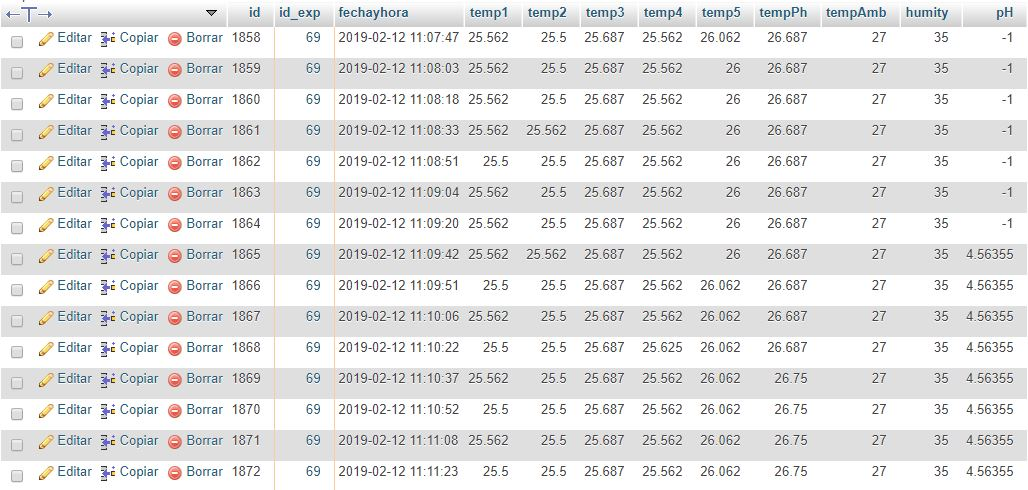
\includegraphics[scale=0.5]{Pruebas/Inserciones.jpg}
    \caption{Captura de mediciones realizadas para la prueba de velocidad}
    \label{fig:pruebasdeInsercion}
\end{figure}
\begin{figure}[H]
    \centering
    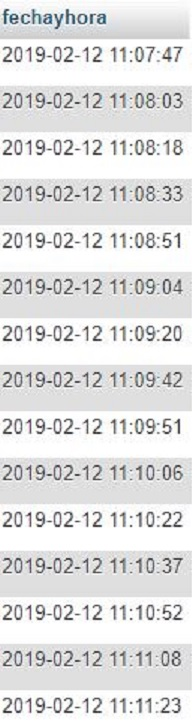
\includegraphics[scale=0.5]{Pruebas/InsercionesZOOM.jpg}
    \caption{Acercamiento de ``fechayhora'' de la tabla de mediciones de pruebas de velocidad}
    \label{fig:pruebasdeInsercionFechayHora}
\end{figure}
\par
Luego, mediante la herramienta \textit{Postman}, fueron realizados tres experimentos. Estos consisten en realizar la consulta de obtención de mediciones a la REST API. En la Figura \ref{fig:pruebasdeConsulta} se presentan los resultados, donde puede evidenciarse una demora con duraciones entre 15 ms y 94 ms para obtener la respuesta. A partir de este rango de tiempo para la respuesta, se asume a la obtención de datos de la \textit{REST API} como excelente para su propósito.
\begin{figure}[h]
    \centering
    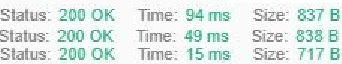
\includegraphics[scale=1]{Pruebas/postman3en1b.jpg}
    \caption{Captura de consulta de mediciones para la prueba de velocidad}
    \label{fig:pruebasdeConsulta}
\end{figure}

\par
Concretadas estas pruebas, se evidenció que el valor mínimo posible para el intervalo de medición de temperatura es de 22 segundos. Ya que el valor de medición de temperatura mínimo definido para el sistema es de 60 segundos, se asumen satisfactorios los resultados, cumpliendo de esta manera el requerimiento no funcional que motivó la misma.

\subsection{Pruebas de campo}
\par En este apartado se exponen un conjunto de pruebas experimentales realizadas con el fin de demostrar que los resultados obtenidos por el sistema en el análisis y optimización de insumos cumplen los requerimientos. 

    \subsection{Metodología de pruebas}
        % ---- TERMO -----
        \par Con la finalidad de ejecutar las pruebas se utilizó como macerador un termo\footnote{Termo, adaptación doméstica de un frasco de Dewar} de forma cilíndrica con capacidad volumétrica de 2,5 litros. Al mismo se le realizaron orificios pasantes de forma de incorporar en su interior los sensores de temperatura sumergibles, (Figura \ref{fig:ConstrucMacerador}).
        
        \par En cuanto a la cantidad y ubicación de los sensores dentro del tanque de macerado, considerando el requerimiento RNF006, se buscó la mínima configuración que permitiese realizar mediciones que cubran el radio y la altura del mismo. Para este diseño se utilizó el análisis presentado en el apartado \ref{colocacionDeSensores}. Se tomó como punto de partida la utilización de los vértices de un polígono de tres lados circunscrito en un círculo (vista superior del tanque de maceración, Figura \ref{fig:SensoresEnTanque}, vértices \textbf{A}, \textbf{B} y \textbf{C}). De forma de obtener temperaturas representativas de las distintas profundidades del tanque, se ubicó cada sensor en un vértice desplazado en altura, manteniendo los mismos a distancias verticales equidistantes. De forma adicional, se incorporó un cuarto sensor, centro \textbf{O} del polígono, ubicado en el centroide del tanque. Véase el resultado de la distribución de los sensores \textbf{A'}, \textbf{B'}, \textbf{C'} y \textbf{O'} en la Figura \ref{fig:SensoresEnTanque}.

        \begin{figure}[h]
            \centering
            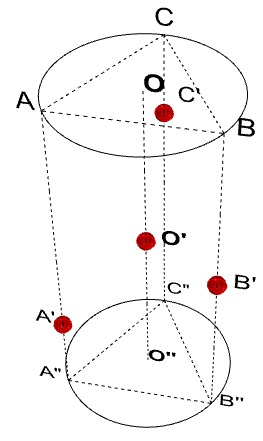
\includegraphics[scale=0.5]{Pruebas/UbicacionSensoresEnTanque-04.jpeg}
            \caption{Esquema representativo de la ubicación de los sensores en el tanque de maceración de forma cilíndrica. La distribución de los sensores A', B', C' y O' (color rojo) yacen en tres niveles de altura distintos, dividiendo el volumen en cuatro secciones verticales de igual tamaño. Para este caso, la altura de los sensores B' y O' se corresponde con el segundo nivel de altura. En vista en planta, los sensores A', B' y C' coinciden con los vértices de un triángulo equilátero (A, B y C) y el sensor O' con el centro de esta figura (O) que se encuentra circunscrita en el cilindro.}
            \label{fig:SensoresEnTanque}
        \end{figure}
        
        \par Los sensores introducidos fueron fijados por medio de pegamento de base siliconada en las posiciones antes indicadas (Figura \ref{fig:ConstrucMacerador}). Para separar los sensores de los bordes del macerador, se utilizaron piezas de poliestireno expandido, que fueron fijadas entremedio de cada sensor de temperatura y el borde interno del termo.
        Con la finalidad de disminuir la pérdida de calor producida por las perforaciones realizadas para introducir estos sensores, se procedió a aplicar sellador siliconado  en los orificios.
        
        \par El termo utilizado cuenta con pico vertedor. El mismo facilita la extracción de muestras sin la necesidad de exponer toda la templa a la temperatura ambiente que produciría la disminución de temperatura y, por tanto, la alteración del experimento.
        
        \par Durante la construcción del macerador, se identificó que el mismo perdía temperatura a un ritmo mayor al aceptable. Por tanto, se procedió a colocar el macerador dentro de un bolso térmico de manera de aumentar el aislamiento. (Figura \ref{fig:ConstrucAislamTerm}).
        
        % ------- pH --------
        \par El sensor de pH fue calibrado para cada una de las maceraciones de prueba realizadas, requerimiento para mejorar la precisión de las mediciones obtenidas señalado en la subsección \ref{subseccionConsideracionesPreviasSensores}.
        
        \par La calibración del sensor de pH consiste en la aplicación de una secuencia de pasos, en los que se ajusta un parámetro mediante software, durante una medición de pH de una solución con un valor estable conocido con el objetivo de mejorar el resultado obtenido. Para este procedimiento, son utilizadas dos soluciones \textbf{buffers} \footnote{Solución química que posee un valor de pH conocido.} cuyos valores (mínimo y máximo) encierran al rango de valores a ser medidos en el experimento. En este caso, el rango de medición varía entre 5 y 6, por tanto, se utilizaron soluciones con valores de pH de 4 y 10, véase Figura \ref{fig:CalibrPhimetro} del Anexo. Luego, esta secuencia inicia con la inmersión de la sonda dentro de la solución \textbf{buffer}. A continuación, se realiza una medición, y se ajusta el resultado mediante un parámetro para este fin. Finalmente, se repite este procedimiento entre las dos soluciones hasta arribar a un valor de ajuste que permita obtener un resultado lo más preciso posible para ambas.
        
        \par Las mediciones de pH se realizaron a partir de una muestra alojada en un recipiente de aluminio refrigerado (figura \ref{fig:MedicPH}) para disminuir la temperatura de la solución a la temperatura de calibración (ver Tabla \ref{tablePhvsTemp}). De forma adicional, dentro del recipiente se alojó un sensor de temperatura con el fin de indicar la temperatura de la templa al momento de la medición de pH.
        
        % ------ Temperatura ------
        \par Al comienzo de un experimento de macerado debe realizarse una infusión entre agua y malta. Ambas en cantidades que deben ser medidas, y en el caso del agua hallarse a una temperatura inicial. Con el fin de medir la cantidad de malta se utilizó una balanza y un recipiente destinado a contenerla. Luego, para calentar y fraccionar el agua utilizada en las pruebas, se empleó una olla de acero inoxidable de cinco litros y un recipiente medidor de un litro. La cantidad y temperatura del agua utilizada en cada uno de los experimentos fue acorde a las indicaciones provistas por la aplicación, pantalla de detalle de maceración, (mencionado en la subsección \ref{DescripPantallaDetalleMaceración}).
        
        \par En cuanto a la identificación de la temperatura inicial del agua, se utilizó una funcionalidad provista por el sistema. En forma conjunta, esta funcionalidad consiste de un sensor de temperatura destinado a este fin y la utilización de la función para la realización de mediciones ``informar valores actuales'', la cual puede encontrarse en la pantalla principal de la aplicación.
        
        \par En particular, para las pruebas con maceraciones escalonadas, para que un cierto volumen de maceración aumente su temperatura a un valor objetivo (escalón de temperatura) debe ser agregada agua a temperatura de hervor. La cantidad de agua caliente que debe ser incorporada al mosto para producir un salto de temperatura es provista por la aplicación en la pantalla ``detalle de maceración'' (mencionado en la subsección \ref{DescripPantallaDetalleMaceración}).
        
        % ------ Densidad ----
        \par Al final de cada experimento de maceración debe ingresarse, en la aplicación, el valor correspondiente a la densidad final obtenida del proceso. La medición de la misma fue realizada mediante la utilización de un densímetro, de escala 1 - 1,1 [$kg/m^3$], y una probeta, de 170 [$cm^3$]. El procedimiento consiste en la toma de una muestra del mosto que es incorporada dentro de la probeta, finalmente, se introduce el densímetro en la probeta para realizar la medición correspondiente.
        
        % ------ Mediciones ----
        \par Para la realización de los experimentos se optó por utilizar intervalos de medición de 1 minuto para la medición de temperatura y 10 minutos para la obtención de la medida de pH. Si bien el sistema soporta mayor frecuencia de medición de pH, la limitante del volumen del recipiente empleado no permite obtener una cantidad de templa de la cual se puedan extraer demasiadas muestras sin que el total de estas extracciones afecte al resultado final. La cantidad de pruebas se definieron acorde a la realización de diez experimentos por cada tipo de maceración planteada. Es a partir de tres experimentos, que el sistema comienza a realizar ajustes sobre el cálculo de insumos. Luego, con diez experimentos es posible observar el ajuste de este valor.
        
        % ---- Grano ----
        \par La malta utilizada para todos los experimentos proviene del mismo lote, y es resguardada en las mismas condiciones. De esta manera puede asegurarse que cualquier cambio de rendimiento obtenido se debe únicamente a la cantidad de insumo utilizado. Definiendo así, las mismas condiciones para todos los experimentos.
        
        En el Anexo \ref{AnexoFotografias} se ubican una serie de imágenes relacionadas a la construcción del sistema y a los procedimientos involucrados en el proceso de maceración.
        
        \subsection{Recetas y tipos de maceración utilizadas}
        
        \par Para llevar a cabo los experimentos se planificaron las siguientes maceraciones:
        \hfill \break
        \hfill \break
        \begin{longtable}{p{0.6cm} p{0.6cm} p{12.8cm}}

        \endfirsthead
 
        \endhead
 
        \endfoot
 
        \endlastfoot


        \multicolumn{3}{l}{\textbf{Pilsen Lager - Simple}}\\
        & & \\
        & \multicolumn{2}{l}{Tipo de Maceración: Simple} \\
        & \multicolumn{2}{l}{Volumen: 2 litros}  \\
        & \multicolumn{2}{l}{Densidad específica deseada: 1.070} \\
        & & \\
        & \multicolumn{2}{l}{Granos:} \\
        & & Nombre: Pilsener \\
        & & Porcentaje de utilización: 100\% \\
        & & Extracto Potencial: 80\% \\
        & & \\
        & \multicolumn{2}{l}{Intervalos:} \\
        & & Duración: 60 minutos \\
        & & Temperatura objetivo: 65°C \\
        & & Desvío de temperatura tolerado: ±3°C \\
        & & pH: 5.4 \\
        & & Desvío de pH tolerado: ±0.2 \\
        & & \\
        & & \\
        \multicolumn{3}{l}{\textbf{Pilsen Lager - Escalonada}}\\
        & & \\
        
        & \multicolumn{2}{l}{Tipo de Maceración: Escalonada} \\
        & \multicolumn{2}{l}{Volumen: 2 litros}  \\
        & \multicolumn{2}{l}{Densidad específica deseada: 1.070} \\
        & & \\
        & \multicolumn{2}{l}{Granos:} \\
        & & Nombre: Pilsener \\
        & & Porcentaje de utilización: 100\% \\
        & & Extracto Potencial: 80\% \\
        & & \\
        & \multicolumn{2}{l}{Intervalos:} \\
        & & Duración: 20 minutos \\
        & & Temperatura objetivo: 45°C \\
        & & Desvío de temperatura tolerado: ±3°C \\
        & & pH: 5.4 \\
        & & Desvío de pH tolerado: ±0.2 \\
        & & \\
        & & Duración: 20 minutos \\
        & & Temperatura objetivo: 55°C \\
        & & Desvío de temperatura tolerado: ±3°C \\
        & & pH: 5.4 \\
        & & Desvío de pH tolerado: ±0.2 \\
        & & \\
        & & Duración: 20 minutos \\
        & & Temperatura objetivo: 65°C \\
        & & Desvío de temperatura tolerado: ±3°C \\
        & & pH: 5.4 \\
        & & Desvío de pH tolerado: ±0.2 \\

        \end{longtable}
    
    \subsection{Valores calculados para cada receta}
    %\hfill \break
    \par A continuación se visualizan los valores calculados por la aplicación para conocer la cantidad de insumos necesaria para realizar la maceración según la planificación correspondiente.
    %\par La cantidad de insumos ajustados se empieza a visualizar a partir de la tercer fila, acorde a la regla de negocio planteada en el capítulo de \ref{}.
    
        \subsubsection{Pilsen Lager - Simple}
        
        \begin{longtable}{|p{2.7cm}|p{2.7cm}|p{2.7cm}|p{2.7cm}|p{2.7cm}|}
        \hline
        Experimentos & Rendimiento utilizado & Insumos utilizados & Rendimiento obtenido & Insumos ajustados\\
        \endfirsthead
        
        \endhead
 
        \endfoot
        
        \hline
        \caption{Tabla de resultados Pilsen Lager simple\label{tab:ResultadosPilsenSimple}}\\
        \endlastfoot
        \hline
             \multicolumn{1}{|c|}{1} & \multicolumn{1}{c|}{70\%} & \multicolumn{1}{c|}{0.36 Kg.} &\multicolumn{1}{c|}{60.13\%} &\multicolumn{1}{c|}{-} \\
             \hline
             \multicolumn{1}{|c|}{2} & \multicolumn{1}{c|}{70\%}  & \multicolumn{1}{c|}{0.36 Kg.} &\multicolumn{1}{c|}{61.16\%} &\multicolumn{1}{c|}{-} \\
             \hline
             \multicolumn{1}{|c|}{3} & \multicolumn{1}{c|}{70\%} & \multicolumn{1}{c|}{0.36 Kg.} &\multicolumn{1}{c|}{62.54\%} &\multicolumn{1}{c|}{0.37356 Kg.} \\
             \hline
             \multicolumn{1}{|c|}{4} & \multicolumn{1}{c|}{62.54\%}  & \multicolumn{1}{c|}{0.4 Kg.} &\multicolumn{1}{c|}{63.75\%} &\multicolumn{1}{c|}{0.37777 Kg.} \\
             \hline
             \multicolumn{1}{|c|}{5} & \multicolumn{1}{c|}{63.75\%}  & \multicolumn{1}{c|}{0.37777 Kg.} &\multicolumn{1}{c|}{64.89\%} &\multicolumn{1}{c|}{0.38221 Kg.} \\
             \hline
             \multicolumn{1}{|c|}{6} & \multicolumn{1}{c|}{64.89\%}  & \multicolumn{1}{c|}{0.38221 Kg.} &\multicolumn{1}{c|}{66.17\%} &\multicolumn{1}{c|}{0.39111 Kg.} \\
             \hline
             \multicolumn{1}{|c|}{7} & \multicolumn{1}{c|}{66.17\%}  & \multicolumn{1}{c|}{0.39111 Kg.} &\multicolumn{1}{c|}{66.78\%} &\multicolumn{1}{c|}{0.37673 Kg.} \\
             \hline
             \multicolumn{1}{|c|}{8} & \multicolumn{1}{c|}{66.78\%}  & \multicolumn{1}{c|}{0.37673 Kg.} &\multicolumn{1}{c|}{66.99\%} &\multicolumn{1}{c|}{0.36486 Kg.} \\
             \hline
             \multicolumn{1}{|c|}{9} & \multicolumn{1}{c|}{66.99\%}  & \multicolumn{1}{c|}{0.36486 Kg.} &\multicolumn{1}{c|}{67.14\%} &\multicolumn{1}{c|}{0.36401 Kg.} \\
             \hline
             \multicolumn{1}{|c|}{10} & \multicolumn{1}{c|}{67.14\%} & \multicolumn{1}{c|}{0.36401 Kg.} &\multicolumn{1}{c|}{67.48\%} &\multicolumn{1}{c|}{0.37286 Kg.} \\
             \hline
        
        \end{longtable}
        
    
 \subsubsection{Pilsen Lager - Escalonada}
        \begin{longtable}{|p{2.7cm}|p{2.7cm}|p{2.7cm}|p{2.7cm}|p{2.7cm}|}
        \hline
        Experimentos & Rendimiento utilizado & Insumos utilizados & Rendimiento obtenido & Insumos ajustados\\
        \endfirsthead
        
        \endhead
 
        \endfoot
        
        \hline
        
        \caption{Tabla de resultados Pilsen Lager escalonada\label{tab:ResultadosPilsenEscalonada}}\\
        \endlastfoot
        
        \hline
             \multicolumn{1}{|c|}{Experimentos} & \multirow{1}{2cm}{Rendimiento Utilizado} &\multirow{1}{2cm}{Insumos Utilizados}  & \multirow{1}{2cm}{Rendimiento Obtenido} &\multirow{1}{2cm}{Insumos Ajustados}\\
             & & & &\\
             \hline
             \hline
             \multicolumn{1}{|c|}{1} & \multicolumn{1}{c|}{70\%} & \multicolumn{1}{c|}{0.36 Kg.} &\multicolumn{1}{c|}{51.92\%} &\multicolumn{1}{c|}{-} \\
             \hline
             \multicolumn{1}{|c|}{2} & \multicolumn{1}{c|}{70\%}  & \multicolumn{1}{c|}{0.36 Kg.} &\multicolumn{1}{c|}{62.2\%} &\multicolumn{1}{c|}{-} \\
             \hline
             \multicolumn{1}{|c|}{3} & \multicolumn{1}{c|}{70\%} & \multicolumn{1}{c|}{0.36 Kg.} &\multicolumn{1}{c|}{65.3\%} &\multicolumn{1}{c|}{0.37356 Kg.} \\
             \hline
             \multicolumn{1}{|c|}{4} & \multicolumn{1}{c|}{62.54\%}  & \multicolumn{1}{c|}{0.37356 Kg.} &\multicolumn{1}{c|}{64.27\%} &\multicolumn{1}{c|}{0.36529 Kg.} \\
             \hline
             \multicolumn{1}{|c|}{5} & \multicolumn{1}{c|}{62.97\%}  & \multicolumn{1}{c|}{0.36529 Kg.} &\multicolumn{1}{c|}{65.3\%} &\multicolumn{1}{c|}{0.36828 Kg.} \\
             \hline
             \multicolumn{1}{|c|}{6} & \multicolumn{1}{c|}{63.44\%}  & \multicolumn{1}{c|}{0.36828 Kg.} &\multicolumn{1}{c|}{74.66\%} &\multicolumn{1}{c|}{0.40727 Kg.} \\
             \hline
             \multicolumn{1}{|c|}{7} & \multicolumn{1}{c|}{65.31\%}  & \multicolumn{1}{c|}{0.40727 Kg.} &\multicolumn{1}{c|}{70.49\%} &\multicolumn{1}{c|}{0.38094 Kg.} \\
             \hline
             \multicolumn{1}{|c|}{8} & \multicolumn{1}{c|}{66.05\%}  & \multicolumn{1}{c|}{0.38094 Kg.} &\multicolumn{1}{c|}{72.57\%} &\multicolumn{1}{c|}{0.38705 Kg.} \\
             \hline
             \multicolumn{1}{|c|}{9} & \multicolumn{1}{c|}{66.86\%}  & \multicolumn{1}{c|}{0.38705 Kg.} &\multicolumn{1}{c|}{68.41\%} &\multicolumn{1}{c|}{0.36461 Kg.} \\
             \hline
             \multicolumn{1}{|c|}{10} & \multicolumn{1}{c|}{67.03\%} & \multicolumn{1}{c|}{0.36461 Kg.} &\multicolumn{1}{c|}{70.49\%} &\multicolumn{1}{c|}{0.37341 Kg.} \\
             \hline
        
    \end{longtable}
    
    \subsection{Resultados obtenidos}
        \par Para cada receta realizada se muestran las gráficas de promedio de temperatura y pH obtenidas por la aplicación. Las mismas se presentan en el Anexo \ref{GraficasPruebasCampo}.
    
    \subsection{Evaluación}
        \par En la anterior subsección se evidenció que el ajuste de la cantidad de insumos realizada por el sistema produce resultados correctos, esto es, cuando el valor de rendimiento es menor al deseado incrementa la cantidad de granos de manera de compensar este sub-rendimiendo, y lo mismo ocurre en caso contrario con un sobre-rendimiento. Esta compensación representa el objetivo de esta funcionalidad, la cual es asistir al productor a partir de una herramienta de optimización de insumos en función de un ajuste utilizando el rendimiento del equipo.
        
        \par Cabe señalar que si bien pueden parecer reducidos los cambios en los valores de insumo, los mismos corresponden a un preparado de un volumen reducido. Estos cambios crecerán en forma proporcional al tamaño del preparado, constituyéndose en valores más significativos conforme a este incremento, dado que, el comportamiento del sistema y los cálculos realizados son linealmente proporcionales al volumen de producción.
        
        \par Por tanto, puede concluirse que esta funcionalidad del sistema se comporta de la manera esperada, y por tanto, correcta. 